\documentclass[../ai_in_finance]{subfiles}
\usepackage[margin=1in]{geometry}
\usepackage{tikz}
\usetikzlibrary{positioning}
\usepackage{amsmath}
\usepackage{amssymb}
\usepackage{booktabs}
\usepackage{floatrow}
\usepackage{draftwatermark}

\SetWatermarkText{Wulin.Suo@Queensu.ca}
\SetWatermarkScale{1.4}
\SetWatermarkColor{gray!35}
\SetWatermarkAngle{45}

\usepackage{makeidx}
\makeindex

\begin{document}

\chapter{Insurance and Actuarial Modeling}

\section{Introduction}

In August 1992, Hurricane Andrew crossed southern Florida and destroyed, alongside tens of thousands of homes, the insurance industry's confidence in its own loss estimates. Insurers had priced Florida windstorm coverage from a few decades of loss experience that happened to contain no direct hit on a major metropolitan area; Andrew produced insured losses several times larger than the industry's models had contemplated, and roughly a dozen insurers were rendered insolvent by a single storm. The failure was not one of underwriting discipline but of method: historical claims experience, the industry's traditional basis for pricing, is structurally silent about events larger than any it happens to contain. Out of that failure grew the modern catastrophe-modeling industry, simulation-based, physics-informed, and data-hungry, and with it the broader lesson this chapter develops: insurance is, more than any other business in this book, a business of estimating loss distributions, and every advance in how loss distributions are estimated eventually becomes an advance in how insurance is priced, reserved, and supervised.

Insurance deserves a chapter of its own in a book about artificial intelligence in finance for two reasons. First, it is enormous, by assets, by premium volume, and by employment of the quantitatively-trained people this book addresses, and its analytical core, actuarial science\index{actuarial science}, is the oldest data science in finance: actuaries were fitting frequency and severity distributions to loss data a century before the term ``machine learning'' existed. Second, its structure makes the AI questions unusually crisp. An insurer prices a contract before knowing what it will cost, observes rich behavioral data about its customers, adjudicates millions of claims a year, and does all of this inside one of the most consumer-protective regulatory perimeters in finance, so every theme this book has developed, predictive modeling, text and image data, fraud detection, explainability, and fairness, arrives here simultaneously and with unusually high stakes.

The chapter's central claim, the same asymmetry Chapter 10 found in operational risk, is worth stating up front. Machine learning does not replace the actuarial core; it feeds and sharpens it at every point where the data is \emph{granular} or \emph{unstructured}: driver-level sensor streams instead of rating-cell averages, claim-level features instead of aggregate triangles, document and image inputs instead of questionnaires, and interactions no multiplicative rating plan anticipates. The classical structure, frequency times severity, credibility, the development triangle, the filed rating plan, remains the layer that regulators audit and balance sheets are built on. Each section below therefore pairs the two explicitly: the classical calculation first, then a worked example of the machine-learning layer that now sits underneath it, each small enough to check by hand.

The chapter proceeds from economics to methods to frontiers, and Figure~\ref{fig:ins-value-chain} maps where AI enters along the way. It first establishes what makes insurance structurally different and how an insurer actually makes money, then develops the classical quantitative core, frequency-severity pricing, the one-way-rating failure that motivated generalized linear models, credibility theory, and chain-ladder reserving, each with a worked example a reader can check by hand. It then works through where machine learning genuinely changes each function, pricing, telematics, claims, reserving, underwriting, before widening to the balance-sheet topics, life and health insurance, asset-liability management, catastrophe risk and parametric transfer, and solvency capital, that connect insurance to the valuation, portfolio, and risk chapters earlier in this book. It closes where insurance regulation now concentrates: fairness, price optimization, and proxy discrimination in AI-driven pricing.

\begin{figure}[htbp]
\centering
\begin{lrbox}{\bookmeasuredbox}
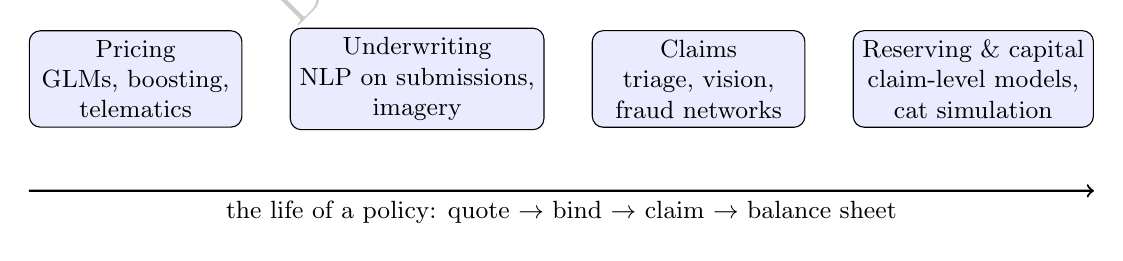
\begin{tikzpicture}[node distance=4mm, every node/.style={font=\small}]
\node[draw, rounded corners, fill=blue!8, minimum width=2.7cm, minimum height=1.0cm, align=center] (price) {Pricing\\ GLMs, boosting,\\ telematics};
\node[draw, rounded corners, fill=blue!8, minimum width=2.7cm, minimum height=1.0cm, align=center, right=6mm of price] (uw) {Underwriting\\ NLP on submissions,\\ imagery};
\node[draw, rounded corners, fill=blue!8, minimum width=2.7cm, minimum height=1.0cm, align=center, right=6mm of uw] (clm) {Claims\\ triage, vision,\\ fraud networks};
\node[draw, rounded corners, fill=blue!8, minimum width=2.7cm, minimum height=1.0cm, align=center, right=6mm of clm] (res) {Reserving \& capital\\ claim-level models,\\ cat simulation};
\draw[->, thick] ([yshift=-8mm]price.south west) -- ([yshift=-8mm]res.south east) node[midway, below] {the life of a policy: quote $\rightarrow$ bind $\rightarrow$ claim $\rightarrow$ balance sheet};
\end{tikzpicture}
\end{lrbox}
\ifdim\wd\bookmeasuredbox<0.65\linewidth
\setlength{\bookcapwidth}{0.65\linewidth}
\else
\setlength{\bookcapwidth}{\wd\bookmeasuredbox}
\fi
\ffigbox[\bookcapwidth]{
\usebox{\bookmeasuredbox}
}{
\caption{AI across the insurance value chain. Every stage feeds a filed rate or a regulated capital number, which is what makes governance structural here.}
\label{fig:ins-value-chain}
}
\end{figure}

\section{The Economics of Insurance}

An insurer sells a promise and invests the proceeds, which makes its economics unlike any other financial firm's.

\subsection{What Makes Insurance Different}
\label{sec:ins-fundamentals}

Insurance inverts the production cycle of almost every other business: the price is collected first and the cost of goods sold, the claims, is discovered afterward, sometimes decades afterward. Everything distinctive about the industry follows from this inversion. Profitability cannot be read off current revenue; it must be \emph{estimated}, by forecasting the ultimate cost of claims already incurred (the reserving problem of Section~\ref{sec:ins-reserving}) and of contracts still in force. The product is a promise, so the industry is regulated primarily for solvency, an insurer must demonstrably be able to pay claims years away, and secondarily for fairness in pricing, since coverage is often practically or legally mandatory.

The economic engine is risk pooling\index{risk pooling}, and it is worth seeing the engine's mathematics once, because a single calculation explains why the industry exists. Suppose each of $n$ independent policies produces an annual loss with mean $\mu = \$720$ and standard deviation $\sigma = \$3{,}000$, a violently uncertain individual prospect, with a coefficient of variation of $3{,}000/720 \approx 417\%$. The pooled loss across $n = 10{,}000$ such policies has mean $n\mu = \$7.2$ million but standard deviation only $\sigma\sqrt{n} = \$300{,}000$, a coefficient of variation of $4.17\%$: aggregation has shrunk relative uncertainty by a factor of $\sqrt{n} = 100$. A loss more than $10\%$ above expectation is a $z = 2.4$ event, roughly a $0.8\%$ probability under a normal approximation. Individually unpredictable losses have become collectively predictable, and \emph{that predictability, not risk-bearing appetite, is the product}: the insurer sells the law of large numbers, retail. The calculation also displays its own failure mode, which Section~\ref{sec:ins-cat} takes up: everything above assumed independence, and a hurricane, correlating a hundred thousand claims into one event, deletes the $\sqrt{n}$.

Two classic frictions limit the engine. Adverse selection\index{adverse selection} is the tendency of higher-risk customers to seek more coverage, which the insurer combats with underwriting and risk-based pricing; moral hazard\index{moral hazard} is the tendency of insured parties to take more risk once covered, combated with deductibles and coverage limits. Both frictions are, at bottom, information problems, which is precisely why an industry built on them has always been an early adopter of any technology that reduces information asymmetry, from the mortality table to the telematics device of Section~\ref{sec:ins-telematics}.

The reader will recognize the analytical machinery immediately. An insurance portfolio's annual loss is a compound frequency-severity sum, exactly the loss distribution approach Chapter 10 developed for operational risk, and for the same reason: both fields face losses that arrive as a random number of events of random size. The historical direction of travel, worth appreciating, is that operational risk borrowed this machinery \emph{from} actuarial science, not the other way around.

\subsection{How an Insurer Makes Money: Float and the Combined Ratio}
\label{sec:ins-economics}

Before pricing a single policy, it pays to understand the business model the prices feed. An insurer's operating result has two engines, illustrated in Figure~\ref{fig:ins-cycle}. The underwriting engine is summarized by the combined ratio\index{combined ratio}: losses plus expenses, divided by premiums. A combined ratio below $100\%$ means the insurance operation is profitable in its own right. The investment engine runs on float\index{float (insurance)}: because premiums arrive before claims are paid, the insurer continuously holds a large pool of policyholder money, the loss reserves of Section~\ref{sec:ins-reserving} plus unearned premiums, which it invests for its own account.

A worked example shows how the engines combine. An insurer writes \$100 million of premium, incurs \$65 million of losses (a $65\%$ loss ratio) and \$30 million of expenses (a $30\%$ expense ratio), for a combined ratio of $95\%$ and an underwriting profit of \$5 million. It also holds \$150 million of float invested at a $4\%$ yield, earning \$6 million, so total pre-tax operating income is \$11 million, a $22\%$ return on its \$50 million of supporting capital. Now rerun the year with a $103\%$ combined ratio: underwriting loses \$3 million, yet the insurer still earns \$3 million overall, because the \$3 million underwriting loss is simply the \emph{cost} of holding \$6 million worth of investable float, cheaper than any other funding the insurer could raise. This arithmetic, made famous by Berkshire Hathaway's shareholder letters, explains a great deal of observed industry behavior: why insurers will write at small underwriting losses in competitive markets, why reserving accuracy (which determines how much float there really is, and for how long) is a first-order economic question rather than an accounting formality, and why the asset-liability topics of Section~\ref{sec:ins-alm} belong in the same chapter as pricing.

It also locates, before any model appears, exactly where machine learning can move the profit needle, because the combined ratio has only two components to move. Every AI application in this chapter attacks one of them: better risk selection and pricing (Sections~\ref{sec:ins-ml-pricing}--\ref{sec:ins-telematics}) and earlier fraud detection (Section~\ref{sec:ins-claims}) lower the \emph{loss} ratio, while automated claims handling, straight-through processing, and NLP-driven underwriting (Sections~\ref{sec:ins-claims} and~\ref{sec:ins-underwriting}) lower the \emph{expense} ratio, and on the worked book each point of combined ratio is worth \$1 million of premium, pre-tax, every year. That is the business case that funds the industry's AI investment, and it disciplines the evaluation standard used throughout this chapter: an insurance model is judged by the ratio points it moves, not by its accuracy in the abstract.

\begin{figure}[htbp]
\centering
\begin{lrbox}{\bookmeasuredbox}
% Tightened from "5mm and 12mm" / below=14mm: the gaps, not the boxes, were
% what made this diagram loose, and the drop to the income box also set the
% height of the elbow carrying the "combined ratio" label on the left.
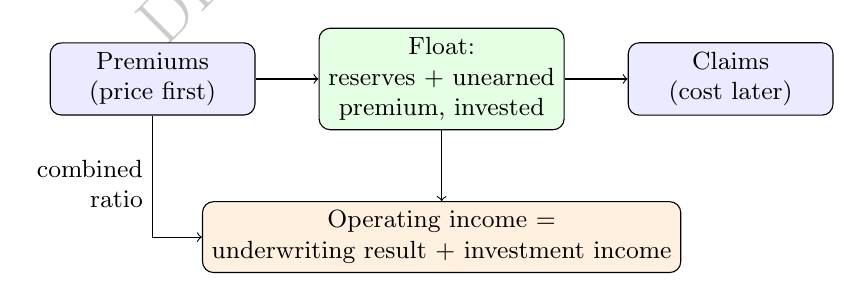
\begin{tikzpicture}[node distance=4mm and 8mm, every node/.style={font=\small}]
\node[draw, rounded corners, fill=blue!8, minimum width=2.6cm, minimum height=0.9cm, align=center] (prem) {Premiums\\ (price first)};
\node[draw, rounded corners, fill=green!10, minimum width=3.0cm, minimum height=1.1cm, align=center, right=of prem] (float) {Float:\\ reserves + unearned\\ premium, invested};
\node[draw, rounded corners, fill=blue!8, minimum width=2.6cm, minimum height=0.9cm, align=center, right=of float] (claims) {Claims\\ (cost later)};
\node[draw, rounded corners, fill=orange!12, minimum width=3.0cm, minimum height=0.9cm, align=center, below=9mm of float] (income) {Operating income =\\ underwriting result + investment income};
\draw[->] (prem) -- (float);
\draw[->] (float) -- (claims);
\draw[->] (float) -- (income);
\draw[->] (prem.south) |- node[pos=0.28, left, align=right] {combined\\ ratio} (income.west);
\end{tikzpicture}
\end{lrbox}
\ifdim\wd\bookmeasuredbox<0.65\linewidth
\setlength{\bookcapwidth}{0.65\linewidth}
\else
\setlength{\bookcapwidth}{\wd\bookmeasuredbox}
\fi
\ffigbox[\bookcapwidth]{
\usebox{\bookmeasuredbox}
}{
\caption{The inverted production cycle: premiums arrive before claims are paid, and the pool of policyholder money in between, the float, is invested for the insurer's account. Underwriting profitability (the combined ratio) and investment income on float are the business's two engines.}
\label{fig:ins-cycle}
}
\end{figure}

\subsection{The Classical Pricing Baseline: Frequency Times Severity}
\label{sec:ins-pricing}

Suppose an auto insurer must set next year's premium for a policyholder it has never observed have an accident. The classical answer prices the \emph{expected} loss and then loads it for expenses and profit. The pure premium\index{pure premium} is
\begin{equation*}
\text{pure premium} \;=\; \mathbb{E}[N] \times \mathbb{E}[X],
\end{equation*}
expected claim frequency ($N$) times expected claim severity ($X$), and the art of ratemaking is estimating how each component varies with observable characteristics of the risk.

A worked example fixes the mechanics. Suppose the book-wide base rates are a claim frequency of $0.08$ claims per policy-year and a mean severity of \$9{,}000, giving a base pure premium of $0.08 \times 9{,}000 = \$720$. Rating factors enter multiplicatively: suppose young drivers exhibit $1.8$ times the base frequency, urban territories $1.25$ times the base frequency, and urban claims run $1.10$ times the base severity (denser traffic produces more collisions; urban repair and injury costs run higher). A young urban driver's expected frequency is then $0.08 \times 1.8 \times 1.25 = 0.18$ and expected severity $9{,}000 \times 1.10 = \$9{,}900$, for a pure premium of $0.18 \times 9{,}900 = \$1{,}782$, about $2.5$ times the base risk. Loading for a $25\%$ expense ratio and a $5\%$ profit provision, the gross premium solves $\text{premium} \times (1 - 0.25 - 0.05) = \text{pure premium}$, giving $1{,}782 / 0.70 \approx \$2{,}545.71$.

This arithmetic is the skeleton; the instrument that estimates the relativities filling it in is the generalized linear model of the next section, and it is important to be clear about vocabulary before the machine-learning comparison arrives: when the insurance industry says ``traditional pricing,'' it means \emph{GLM-based} pricing. The GLM is not a stepping stone on the way to modern methods; it has been the established standard for decades, and it is the incumbent that machine learning must beat.

\section{Pricing and Claims}

This part covers how a premium is actually set, from the generalized linear model through credibility to telematics, and what happens when a claim arrives.

\subsection{GLM Ratemaking: The Traditional Approach}
\label{sec:ins-glm}

Where do relativities like the $1.8$ and $1.25$ above come from? The tempting answer, compute each factor's relativity from its own marginal experience, one factor at a time, contains a trap important enough to work through numerically, because escaping the trap is precisely what made the generalized linear model the industry's standard.

Consider a portfolio with two rating factors, age (young/experienced) and territory (urban/rural), with exposures and claim counts by cell:

\begin{table}[htbp]
\centering
\begin{lrbox}{\bookmeasuredbox}
\begin{tabular}{lcccc}
\toprule
Cell & Exposure & Claims & Frequency \\
\midrule
Young, urban & 200 & 54 & 0.270 \\
Young, rural & 50 & 9 & 0.180 \\
Experienced, urban & 300 & 45 & 0.150 \\
Experienced, rural & 450 & 45 & 0.100 \\
\bottomrule
\end{tabular}
\end{lrbox}
\ifdim\wd\bookmeasuredbox<0.65\linewidth
\setlength{\bookcapwidth}{0.65\linewidth}
\else
\setlength{\bookcapwidth}{\wd\bookmeasuredbox}
\fi
\floatbox[\capbot]{table}[\bookcapwidth]{
\usebox{\bookmeasuredbox}
}{
\caption{Exposures (policy-years), claim counts, and claim frequencies by rating cell}
\label{tab:ins-oneway}
}
\end{table}

The table was built with an exactly multiplicative structure: a base frequency of $0.100$, a young relativity of $1.8$, and an urban relativity of $1.5$ (check: $0.100 \times 1.8 \times 1.5 = 0.270$). Now compute the relativities the one-way approach recovers. Young drivers overall: $(54+9)/(200+50) = 0.252$; experienced overall: $(45+45)/(300+450) = 0.120$; one-way age relativity $0.252/0.120 = 2.10$, not $1.8$. Urban overall: $(54+45)/(200+300) = 0.198$; rural: $(9+45)/(50+450) = 0.108$; one-way territory relativity $1.833$, not $1.5$. Both are inflated, and for the same reason: young drivers in this portfolio cluster in urban territory ($200$ of $250$ exposures), so the age marginal absorbs part of the territory effect and vice versa, double-counting their overlap. A rating plan built from the one-way factors would charge the young urban cell $2.10 \times 1.833 = 3.85$ times base, against a true relativity of $2.70$, a $43\%$ overcharge, and would symmetrically undercharge the experienced rural cell, with the mispricings then feeding adverse selection as overcharged customers defect to better-priced competitors.

The remedy is simultaneous estimation, and that is precisely what the generalized linear model\index{generalized linear model (GLM)} (GLM) does: a Poisson GLM with a log link fit to claim counts (with exposure as an offset), and a Gamma GLM fit to severities, estimate all relativities \emph{jointly}, each factor's effect measured holding the others fixed, recovering the true $1.8$ and $1.5$ from Table~\ref{tab:ins-oneway} exactly. GLMs extended the ordinary regression of Chapter 6 to the skewed, non-negative distributions insurance data actually exhibit, and their adoption is itself a piece of history worth knowing: spreading from British motor insurance in the 1980s and 1990s, GLM ratemaking displaced the earlier one-way and minimum-bias methods to become the industry's standard classification-ratemaking approach worldwide, the method the Casualty Actuarial Society's own rating monograph presents as the established baseline, so that the phrase ``traditional pricing'' in today's industry debates refers to a method that was, in its time, the data-science modernization. The multiplicative-relativity output is also \emph{filed}: in most U.S. states an insurer must submit its rating plan to a regulator, justify each factor, and use what it filed, a constraint with deep consequences for what follows.

\subsection{Credibility: The Actuary's Bayesian Shrinkage}
\label{sec:ins-credibility}

Between the book-wide rate and the individual risk sits a question the GLM alone does not answer: how much should one policyholder's \emph{own} experience move their price? A commercial fleet with three years of history and one claim exhibits an observed frequency of $1/3 \approx 0.333$ against a class rate of $0.100$; charging either number is plainly wrong, the first because three years of one fleet is noise, the second because it ignores real information. Credibility theory\index{credibility theory}, actuarial science's oldest continuously-used tool, prescribes the blend
\begin{equation*}
\hat f \;=\; Z \times \bar f_{\text{own}} + (1 - Z) \times f_{\text{class}}, \qquad Z = \frac{n}{n + k},
\end{equation*}
where $n$ is the volume of the risk's own experience and $k$ measures how noisy individual experience is relative to how much risks genuinely differ (formally, the ratio of expected process variance to the variance of true means across risks, the B\"uhlmann\index{Buhlmann credibility} formulation). With $n = 3$ years and $k = 12$, the credibility weight is $Z = 3/15 = 0.20$ and the blended frequency $0.20 \times 0.333 + 0.80 \times 0.100 \approx 0.147$: the fleet's bad year moves its rate meaningfully but not catastrophically, and each additional year of clean experience will pull it back.

The reader who has followed this book will recognize the formula three times over. It is Chapter 1's Bayesian updating, the class rate as prior, own experience as likelihood, with $Z$ the posterior weight on the data; it is the shrinkage of Chapter 6's ridge regularization, pulling noisy individual estimates toward a grand mean by an amount that declines as evidence accumulates; and it is structurally the partial pooling that modern hierarchical models perform. Actuaries derived it in the 1910s--1960s because rate regulation forced them to price small risks honestly; machine learning rederived it as regularization half a century later. Credibility is this chapter's cleanest evidence for a claim made in the introduction: actuarial science is not a field awaiting rescue by data science; it is a parallel, older branch of the same subject.

\subsection{From GLMs to Machine Learning in Pricing}
\label{sec:ins-ml-pricing}

The machine-learning question in pricing is therefore precisely posed: the incumbent is not a naive method but the GLM, a decades-refined statistical model with a regulatory apparatus built around it, and ``machine learning versus traditional pricing'' means, concretely, boosted trees versus the GLM. Everything Chapter 6 established about flexible models applies, with one structural twist. Gradient-boosted trees routinely beat a GLM's predictive accuracy on large personal-lines datasets, for the familiar reason: real loss processes contain interactions (age with vehicle power, territory with annual mileage) that a multiplicative model captures only if an actuary thinks to specify them, while a tree ensemble finds them automatically, the same lesson as Section~\ref{sec:ins-glm}'s one-way trap, one level up.

\subsubsection*{A Worked Example: The Interaction a GLM Cannot Price}
\label{sec:ins-interaction}

The claim deserves numbers, and Table~\ref{tab:ins-oneway}'s portfolio provides them with one realistic change. Suppose inexperience is genuinely more dangerous in dense traffic, so the young-urban cell's true frequency is $0.32$ ($64$ claims on $200$ exposures) rather than the multiplicative $0.27$, while the other three cells keep their multiplicative values. No multiplicative model can fit these four cells: multiplicativity forces the young-urban frequency to equal base times young times urban, and the data now violate that. Refitting the Poisson GLM to the modified portfolio shows how the failure actually manifests, which is subtler than simply mispricing the interaction cell. The fitted parameters come back as a base frequency of $0.0977$ with relativities of $2.05$ (young) and $1.57$ (urban): the interaction has \emph{leaked into the marginals}, inflating both, because the young-urban cell dominates the exposure behind each. The fitted model then prices the young-urban cell at $0.315$ against a true $0.320$, only $1.6\%$ light, but overprices young-rural at $0.201$ against a true $0.180$, an $11.4\%$ overcharge on the cell least responsible for the signal, with the experienced cells absorbing smaller distortions. The mispricing lands on the \emph{other} cells, exactly where nobody is looking.

A depth-two decision tree, Chapter 6's simplest nonlinear model, prices all four cells exactly: its first split on age and second on territory partition the portfolio into the four cells themselves, each predicted at its own observed frequency, and a gradient-boosted ensemble reaches the same fit within a few trees. This is the entire GLM-versus-machine-learning pricing debate in a $2 \times 2$ table: the flexible model wins not by magic but by declining to impose a structure the data contradict. On the standard academic benchmark for this comparison, a French motor liability dataset of nearly seven hundred thousand policies (this chapter's closing challenge exercise), the accuracy improvement is consistent and material, and the same result reproduces across insurers' internal books.

\subsubsection*{Where Machine Learning Improves on the Traditional Approach, and Where It Does Not}
\label{sec:ins-beyond-glm}

The interaction is one instance of a general pattern, and it is worth stating precisely where the improvement beyond the traditional approach comes from, because each channel corresponds to a specific limitation of the traditional toolkit, the GLM in pricing, and its counterparts elsewhere in the chapter, rather than to generic ``more power.'' First, \emph{interaction discovery at scale}: an actuary can hand-specify the young-urban term once told about it, but cannot hand-specify the thousands of candidate interactions among dozens of rating variables that a boosted ensemble searches automatically; the ensemble's advantage grows with the width of the rating plan. Second, \emph{nonlinear continuous effects without hand-chosen bins}: a GLM represents driver age through bands or polynomial terms the actuary selects in advance, and the true age curve, steeply falling through the twenties, flat in mid-life, rising again past seventy, is captured only as well as those choices allow, while a tree ensemble learns the curve's shape, including its non-monotonicity, directly from data. Third, \emph{high-cardinality categorical variables}: vehicle model and postcode take thousands of levels that a GLM must manually group (or shrink with Section~\ref{sec:ins-credibility}'s credibility machinery, applied level by level), while tree ensembles and learned embeddings, Chapter 16's representation idea applied to categories, handle them natively. Fourth, and most consequentially, \emph{features the GLM could never build}: a GLM can only consume a tabular feature someone constructed, while the deep-learning methods of Chapters 16 and 17 construct the features themselves, the braking signature inside a telematics stream, the roof condition inside an aerial image, the hazard buried in a broker narrative, which is why the largest practical gains have come less from swapping the GLM out of the filed plan than from feeding it richer inputs it could not have created.

The same four channels recur, in different clothes, wherever this chapter meets a traditional method: claim-level reserving improves on the aggregate triangle by using features the triangle discards (Section~\ref{sec:ins-reserving}); dynamic-lapse models improve on fixed liability durations by learning behavior the bond arithmetic assumes away (Section~\ref{sec:ins-alm}); and cause-enriched mortality models improve on a single index for the same reason. In each case the traditional method is not wrong but \emph{coarse}: it summarizes at a level of aggregation chosen for an era of scarce data and hand computation, and machine learning's contribution is to price, reserve, and hedge at the granularity the data now supports.

Honesty requires the other column. Where the book of business is small, the traditional method's low variance and the credibility machinery win, exactly Chapter 6's bias-variance logic; where the rating plan is narrow and well-understood, there are few interactions left to find; and at the regulatory interface, the GLM's auditability is not a limitation but the point. The mature practice is therefore not replacement but a loop: fit the boosted challenger, let it reveal which interactions and curve shapes the filed GLM is missing, and \emph{distill} those findings back into added GLM terms, so that the filed model captures most of the challenger's lift while remaining a document a regulator can read, with the residual gap between the two serving as a running measure of how much accuracy the filing constraint currently costs.

The structural twist is that the filed-rating-plan constraint converts Chapter 18's explainability discussion from good practice into a binding production requirement. A rate filing must state what the model charges and why, an adverse underwriting decision must often be explained to the applicant under the same family of laws as Chapter 18's adverse-action notices, and several U.S. states now require insurers to demonstrate that models built on nontraditional data do not proxy for prohibited characteristics (Section~\ref{sec:ins-fairness}). The practical industry pattern is therefore a hybrid: machine learning models are used freely where they do not directly set the filed rate, in underwriting triage, retention and demand modeling, claims analytics, and as a challenger benchmark that identifies which interactions the filed GLM should add, while the filed rating plan itself evolves more slowly, with the GLM (or a constrained, explainable boosted model) remaining the regulatory interface. It is this book's recurring accuracy-versus-accountability trade-off, institutionalized more explicitly than anywhere else in finance.

\subsection{Telematics and Usage-Based Insurance}
\label{sec:ins-telematics}

Traditional rating variables, age, territory, vehicle, are all \emph{proxies} for how a person actually drives. Telematics\index{telematics} replaces the proxy with the behavior itself: a device or phone app records mileage, speed, time of day, and the harsh-braking and cornering events that predict collisions, and usage-based insurance prices on that record. This is the cleanest example in this book of AI shrinking an information asymmetry at the individual level: the insurer no longer infers risk from group membership but observes each driver's own revealed behavior.

Continuing the worked example, and making the model explicit rather than waving at it: the insurer's telematics layer is itself a GLM on behavioral features, a log-link frequency model in which the fitted coefficient on harsh-braking events is $-0.163$ per event per hundred miles relative to the rating cell's average. Six months of data show the young urban driver braking harshly two fewer times per hundred miles than their cell's average, so the telematics multiplier is $e^{-0.163 \times 2} = e^{-0.326} \approx 0.722$, converting the age-based relativity of $1.8$ into a personal one of $1.8 \times 0.722 \approx 1.30$. The pipeline is worth seeing whole: raw sensor stream $\rightarrow$ engineered behavioral features (Chapter 17's feature-extraction discipline applied to accelerometer data) $\rightarrow$ a GLM coefficient $\rightarrow$ a rating relativity a regulator can read, machine learning at the granular layer feeding the classical structure at the filed layer, the chapter's central asymmetry in one line of arithmetic. The revised expected frequency is $0.08 \times 1.30 \times 1.25 = 0.13$, the pure premium falls to $0.13 \times 9{,}900 = \$1{,}287$, and the gross premium to $1{,}287/0.70 \approx \$1{,}838.57$, a saving of about \$707, or $27.8\%$, earned by demonstrated behavior rather than demographic reclassification. The same calculation run in reverse explains the business model's controversy: a driver whose data reads badly faces a surcharge no traditional variable would have imposed, and the data itself, continuous location and motion records, raises privacy questions the industry's regulators are still working through. There is also a selection subtlety worth noticing: enrollment is voluntary, and drivers who expect their data to read well are the ones who opt in, so the observed telematics book is not a random sample of the portfolio, a live example of the selection effects Chapter 1 warned inhabit every observational dataset.

\subsection{Claims: Triage, Automation, and Fraud}
\label{sec:ins-claims}

Claims is where an insurer's promises are kept, and it is operationally the most AI-saturated function in the industry. Three applications dominate. \emph{Severity triage} predicts, from the first notice of loss, which claims will become expensive, the injury claim that will develop into litigation, the water leak that will become a mold claim, so that experienced adjusters are assigned early where they change outcomes; this is a regression problem in Chapter 6's sense, with the twist that the target is long-tailed and partially censored (open claims' ultimate costs are not yet known, the same censoring structure as Chapter 15's survival analysis).

A minimal triage model shows the mechanics, in the spirit of Chapter 10's key-risk-indicator example. Suppose a logistic model scores the probability that a new auto claim ultimately exceeds \$50{,}000, from three first-notice features: an attorney is already involved ($+1.6$ on the log-odds), an injury is reported ($+1.3$), and the claim was reported more than a week after the accident ($+0.8$), against an intercept of $-2.2$. Here $\sigma$ is Chapter 6's sigmoid, $\sigma(z) = 1/(1+e^{-z})$, not the standard deviation the same letter denoted in the pooling calculation earlier in this chapter; the two meanings are both standard, and which one is meant is always fixed by whether the symbol is applied to an argument. A claim arriving with attorney and injury flags but promptly reported scores $\sigma(-2.2 + 1.6 + 1.3) = \sigma(0.7) \approx 0.668$; a promptly-adjusted no-injury claim reported late scores $\sigma(-2.2 + 0.8) = \sigma(-1.4) \approx 0.198$. The first is routed to a senior adjuster on day one, the second to straight-through processing, and the model's value is measured not by its accuracy in the abstract but by the outcome difference early senior attention makes on the claims it flags, the same decision-focused evaluation standard this book has applied since Chapter 1. \emph{Straight-through processing} pays simple, well-documented claims automatically, using computer vision on damage photos to estimate repair costs and NLP on claim descriptions to verify coverage, with the operational-risk lesson of Chapter 10 attached: an automated adjudication pipeline is itself a system whose failures (overpayment at scale, systematic wrongful denial) are operational events. \emph{Claims fraud detection} is Chapter 15's machinery transplanted: rare positives, adversarial adaptation, network structure (staged-accident rings share repair shops, clinics, and phone numbers exactly as laundering networks share addresses), and the same precision-recall economics, since every investigated honest claim delays a legitimate payment to a customer who has just suffered a loss.

\section{Reserving, Life, Health, and Assets}

Beyond pricing, an insurer must estimate what it already owes, and manage the assets held against it.

\subsection{Reserving: The Chain Ladder and Its Successors}
\label{sec:ins-reserving}

An insurer's largest liability is typically not claims it knows about but claims it must \emph{estimate}: losses incurred but not yet reported or not yet fully paid. Reserving estimates this liability, and the classical tool, the chain ladder\index{chain ladder}, is worth working once by hand because it is the industry's balance-sheet backbone and a genuinely elegant use of minimal data.

Cumulative paid claims (in \$000s) are arranged by accident year and development age:
\begin{table}[htbp]
\centering
\begin{lrbox}{\bookmeasuredbox}
\begin{tabular}{lccc}
\toprule
Accident year & 12 months & 24 months & 36 months \\
\midrule
Year 1 & 400 & 600 & 660 \\
Year 2 & 450 & 675 & ? \\
Year 3 & 500 & ? & ? \\
\bottomrule
\end{tabular}
\end{lrbox}
\ifdim\wd\bookmeasuredbox<0.65\linewidth
\setlength{\bookcapwidth}{0.65\linewidth}
\else
\setlength{\bookcapwidth}{\wd\bookmeasuredbox}
\fi
\floatbox[\capbot]{table}[\bookcapwidth]{
\usebox{\bookmeasuredbox}
}{
\caption{A cumulative paid-claims development triangle (\$000s)}
\label{tab:ins-triangle}
}
\end{table}

The chain ladder assumes each accident year develops proportionally the way its predecessors did. The 12-to-24-month development factor, estimated from all years observed at both ages, is $(600+675)/(400+450) = 1{,}275/850 = 1.50$; the 24-to-36-month factor is $660/600 = 1.10$. Year 2's ultimate loss is then projected as $675 \times 1.10 = 742.5$ and Year 3's as $500 \times 1.50 \times 1.10 = 825$, so the required reserve, ultimate losses minus amounts already paid, is $(742.5 - 675) + (825 - 500) = 67.5 + 325 = \$392.5$ thousand.

Machine learning enters reserving along two paths. Individual-claim reserving replaces the aggregated triangle with claim-level prediction, typically a gradient-boosted or neural regression of each open claim's remaining cost on the same first-notice features as the triage model above (injury type, attorney involvement, jurisdiction) plus its paid-to-date trajectory, which both improves accuracy and, more importantly, explains \emph{why} reserves move, information a triangle mathematically cannot contain; neural extensions of the chain ladder itself, embedding the development-factor structure inside a network that lets the factors vary with claim characteristics, are the subject of an active actuarial literature (see W\"uthrich and Merz in Further Reading). And the chain ladder's own assumptions, that development patterns are stable across accident years, are exactly what breaks when claims inflation shifts or a new claims process changes settlement speed; the monitoring mindset of Chapter 18, watching for the distribution drift that silently invalidates a fitted model, applies to reserving models with an auditor and a regulator as the interested parties. The stakes are the float arithmetic of Section~\ref{sec:ins-economics}: reserves \emph{are} the float, so systematic under-reserving manufactures phantom profits today at the cost of real insolvency risk later, which is why reserve opinions are among the few statistical estimates in finance that a named, professionally-liable individual must sign.

\subsection{Life Insurance, Mortality, and Longevity}
\label{sec:ins-life}

Everything so far has been property-casualty insurance, short contracts, uncertain frequency and severity. Life insurance inverts the difficulty: the event is certain, only its timing is not, and contracts run for decades, which moves the modeling weight from loss distributions to mortality curves and discounting, the machinery of Chapter 5 applied to human lifetimes.

The atomic calculation is worth seeing once. A one-year term policy pays \$500{,}000 if a policyholder with annual death probability $q = 0.002$ dies during the year. Its expected present value, the net premium, is
\begin{equation*}
q \times B \times v \;=\; 0.002 \times 500{,}000 \times \frac{1}{1.04} \;\approx\; \$961.54,
\end{equation*}
mortality probability times benefit times a one-year discount factor at $4\%$. Every life product, term, whole life, annuities, is an expected-present-value sum of exactly such terms across future years, with level-premium products deliberately overcharging early years to prefund the later ones, creating the enormous, long-duration liabilities that drive Section~\ref{sec:ins-alm}.

The modeling frontier is the mortality curve itself. Mortality improves over time, unevenly by age and cohort, and the standard stochastic model, the Lee-Carter model\index{Lee-Carter model}, is a pleasing reunion of two of this book's tools: it decomposes the age-by-year mortality surface into age profiles and a single time-varying mortality index, a factor extraction in the spirit of Chapter 7's PCA term-structure example, and then forecasts that index as a random walk with drift, Chapter 7's simplest time-series model, applied to human longevity. The symmetric risk is longevity risk\index{longevity risk}: an annuity or pension book loses when people live \emph{longer} than projected, a slow-moving, undiversifiable trend risk that no pooling can remove, transferred in practice through longevity swaps between pension funds and reinsurers. AI's contributions run along both fronts: mortality models enriched with cause-of-death, socioeconomic, and medical-advance information, and accelerated underwriting, replacing the traditional medical exam with predictive models on application data, prescription histories, and, controversially, wearable-device data, moving a weeks-long process toward minutes for low-risk applicants while concentrating the fairness questions of Section~\ref{sec:ins-fairness} on whoever the model routes into full underwriting instead.

\subsection{Health Insurance and Risk Adjustment}
\label{sec:ins-health}

Health insurance runs on different economics from everything above: contracts reprice annually, so the long-tail reserving problem largely disappears, and the dominant friction is not catastrophe but selection, since individuals know far more about their expected medical costs than any application reveals. Modern health-insurance markets manage this with a mechanism that deserves a quantitative reader's attention because it is one of the largest predictive-modeling systems in the world with money attached: risk adjustment\index{risk adjustment}. Regulators pay (or transfer between) insurers according to a model-predicted cost score for each enrollee, so that an insurer attracting sicker members is compensated rather than bankrupted, deliberately removing the incentive to select healthy customers.

The mechanics are a regression with a budget attached, and the risk score is worth computing once, because it \emph{is} a predictive model, an additive regression of next-year cost on demographics and diagnosis indicators, whose fitted coefficients are published as score weights. In the U.S. Medicare Advantage program's HCC framework, a 76-year-old female enrollee might carry a demographic base of $0.45$, plus $0.30$ for diabetes with complications, $0.33$ for heart failure, and $0.22$ for COPD: a risk score of $1.30$, which against a baseline payment of \$10{,}000 brings the insurer \$13{,}000. The incentive problem follows immediately, and it is Goodhart's law, Chapter 10's recurring warning, at industrial scale: the insurer controls the diagnostic coding that feeds the model, so ``upcoding,'' documenting members as sicker than clinically warranted, converts directly into revenue. Adding one unsupported vascular-disease code at $0.13$ lifts the score to $1.43$, worth an extra \$1{,}300 per year, \$130 million across a million-member book per tenth of a point, and both academic estimates and government audits have found aggregate coding-intensity effects of roughly this magnitude, making risk-score integrity one of the largest financial-modeling enforcement areas in the United States.

The AI story is symmetrical, and both sides can be made concrete. On the revenue side, insurers deploy NLP on clinical charts, Chapter 16's machinery, to find \emph{legitimately supportable} diagnoses the treating physician documented but never coded, a use that is lawful and, from the model's perspective, accuracy-improving. On the audit side, the simplest anomaly test is already decisive at scale: if an insurer codes vascular disease in $9\%$ of $10{,}000$ enrollees against a clinically-expected regional prevalence of $6\%$, the excess is $z = (0.09 - 0.06)/\sqrt{0.06 \times 0.94/10{,}000} \approx 12.6$ standard errors, a coding pattern that no plausible casemix difference explains and that flags the book for chart-level review, with Chapter 15's full anomaly-detection machinery taking over from there. The equilibrium is an adversarial modeling contest with a public budget as the stake, and the honest caveat belongs alongside it: a large $z$ proves the coding is anomalous, not that it is fraudulent, and distinguishing genuine casemix from manufactured casemix is the human-review step the statistics only prioritize.

\subsection{The Investment Side: Asset-Liability Management}
\label{sec:ins-alm}

An insurer's balance sheet is a leveraged bond portfolio wrapped around a promise, and managing it is a direct application of Chapter 5's duration machinery with one twist: both sides of the balance sheet move with interest rates. Consider a life insurer with \$110 million of assets of duration $5$ against \$100 million of liabilities of duration $12$ (long-duration promises are the nature of the product), for a surplus of \$10 million. A one-percentage-point \emph{rise} in rates moves assets by $-110 \times 5 \times 1\% = -\$5.5$ million but liabilities by $-100 \times 12 \times 1\% = -\$12$ million, so surplus \emph{rises} to \$16.5 million; a one-point \emph{fall} symmetrically compresses surplus to \$3.5 million. The sign is the point: with liabilities longer than assets, the classic life-insurance posture, it is \emph{falling} rates that quietly impair the industry, which is exactly what a decade of near-zero rates did to life insurers and pension funds worldwide, and why duration-matching, immunization, and the long-dated hedging that Chapter 5's swap and duration tools support are a core insurance discipline rather than an optimization nicety.

The machine-learning layer enters through a fact the calculation above quietly assumed away: a liability's duration is not bond mathematics, because the ``bond'' can walk. Policyholders hold options, to lapse a policy, surrender it for cash, or pour new money into a guarantee, and they exercise them in response to rates: when market rates rise well above the credited rate, surrender becomes attractive; when guarantees are above market, policyholders cling to them. Insurers model this with dynamic lapse\index{dynamic lapse} functions fitted to policyholder-level experience data, a Chapter 6 supervised-learning problem in which the features are the rate gap, policy age, tax penalties, and distribution channel, and the fitted behavior feeds directly back into the liability's \emph{effective} duration. Rerunning the worked example with behavior in it: if a one-point rate rise accelerates lapses enough to shorten effective liability duration from $12$ to $9$, surplus rises only to $110 - 5.5 - (100 - 9) = \$13.5$ million rather than \$16.5 million; if a one-point fall slows lapses and extends duration to $14$, surplus compresses to $110 + 5.5 - (100 + 14) = \$1.5$ million rather than \$3.5 million. Behavior has clipped the good outcome \emph{and} deepened the bad one, the signature of a sold option, Chapter 5's negative convexity with a human exercising it, and the quality of the behavioral model, not the bond arithmetic, is what determines whether the hedge book is sized correctly. The 2022--2023 rate spike gave these models their first genuine out-of-sample test in a generation, the regime-shift risk Chapter 7 warned that models fitted on a calm decade must face.

Two further machine-learning deployments round out the ALM picture. Valuing blocks with embedded guarantees (variable annuities above all) requires nested simulation, economic scenarios outside, valuation runs inside each scenario, whose cost grows multiplicatively; insurers increasingly train neural-network surrogates (Chapter 6's function approximators, in the least-squares Monte Carlo tradition) to replace the inner valuation loop, making hedging programs computable overnight rather than over weeks, with the surrogate's approximation error itself a model risk to be validated per Chapter 10. And the portfolio problem that remains, investing float and surplus against regulatory constraints on asset risk, is Chapter 12's mean-variance machinery under a solvency constraint, which is why insurers became early, large buyers of the private credit assets Chapter 3 described: long, illiquid, yield-bearing assets are a natural match for long, illiquid, \emph{behaviorally-modeled} liabilities.

\section{Capital, Catastrophe, and Fairness}

The tail is where insurance is decided; this part covers catastrophe capital, solvency regulation, and the fairness questions new data raises.

\subsection{Catastrophe Risk, Reinsurance, and Alternative Capital}
\label{sec:ins-cat}

Pooling fails exactly where insurance is needed most: catastrophe losses are not independent across policyholders, a hurricane correlates a hundred thousand claims into one event, so Section~\ref{sec:ins-fundamentals}'s $\sqrt{n}$ arithmetic collapses and the tail must be either modeled and capitalized or transferred. Transfer happens through reinsurance\index{reinsurance}, insurance for insurers, typically written in layers stacked into a tower, as in Figure~\ref{fig:ins-tower}. A worked illustration: a reinsurer sells a \$100 million layer attaching at \$50 million (it pays losses between \$50M and \$150M from a single event). If catastrophe models put the annual probability of an event reaching the layer at $0.04$ and the expected loss within the layer, given such an event, at \$60 million, the layer's expected annual loss is $0.04 \times 60 = \$2.4$ million, a ``rate on line''\index{rate on line} of $2.4\%$ of the limit, before the substantial risk load such correlated, capital-intensive exposure commands. The same exposure increasingly reaches capital markets directly through catastrophe bonds\index{catastrophe bond}, whose investors receive a spread, typically a multiple of the modeled expected loss, for bearing a tail risk largely uncorrelated with the market risk of Chapter 8's portfolios, the diversification argument of Chapter 12 applied to hurricanes.

\begin{figure}[htbp]
\centering
\begin{lrbox}{\bookmeasuredbox}
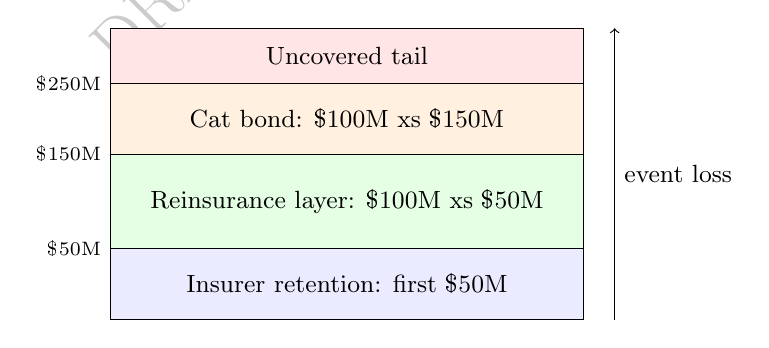
\begin{tikzpicture}[every node/.style={font=\small}]
\draw[fill=blue!8] (0,0) rectangle (6.0,0.9) node[pos=.5] {Insurer retention: first \$50M};
\draw[fill=green!10] (0,0.9) rectangle (6.0,2.1) node[pos=.5] {Reinsurance layer: \$100M xs \$50M};
\draw[fill=orange!12] (0,2.1) rectangle (6.0,3.0) node[pos=.5] {Cat bond: \$100M xs \$150M};
\draw[fill=red!10] (0,3.0) rectangle (6.0,3.7) node[pos=.5] {Uncovered tail};
\draw[->] (6.4,0) -- (6.4,3.7) node[midway, right] {event loss};
\node[left, font=\scriptsize] at (0,0.9) {\$50M};
\node[left, font=\scriptsize] at (0,2.1) {\$150M};
\node[left, font=\scriptsize] at (0,3.0) {\$250M};
\end{tikzpicture}
\end{lrbox}
\ifdim\wd\bookmeasuredbox<0.65\linewidth
\setlength{\bookcapwidth}{0.65\linewidth}
\else
\setlength{\bookcapwidth}{\wd\bookmeasuredbox}
\fi
\ffigbox[\bookcapwidth]{
\usebox{\bookmeasuredbox}
}{
\caption{A catastrophe program as a tower: the insurer retains the first losses, traditional reinsurance covers the middle layers, and a catastrophe bond passes a higher layer to capital-market investors. Each layer's price is quoted as a rate on line: expected annual loss to the layer, plus a risk load, divided by the layer's limit.}
\label{fig:ins-tower}
}
\end{figure}

The models behind these numbers are Hurricane Andrew's institutional legacy: simulation engines that generate tens of thousands of synthetic hurricane seasons or earthquake catalogs, propagate each event's physics over a portfolio of insured locations, and apply engineering damage functions, Monte Carlo over a compound process, once again Chapter 10's architecture at continental scale. AI's contribution is concentrated in the inputs: computer vision on aerial and satellite imagery (Chapter 17's methods) now determines roof geometry, construction type, and post-event damage at the individual-building level, replacing what was once a coarse, self-reported exposure database, and climate-conditioned event generation connects these models to the scenario framework Chapter 8 introduced for climate stress testing.

\subsubsection*{Parametric Insurance and Basis Risk}
\label{sec:ins-parametric}

A structural innovation rounds out the catastrophe toolkit. Parametric insurance\index{parametric insurance} pays a fixed amount when a measured \emph{index} crosses a trigger, wind speed at a reference station, rainfall over a growing season, ground acceleration at a site, rather than indemnifying assessed damage. The payout requires no adjuster, so it arrives in days rather than months, and the product can be sold where claims adjustment is impractical, which is why parametric structures dominate sovereign disaster pools, index-based crop insurance across the developing world, and consumer novelties like flight-delay cover, and why they are a natural match for the satellite and sensor data of Chapter 17.

The price of simplicity is basis risk\index{basis risk (parametric insurance)}: the index and the loss are correlated, not identical. A worked example quantifies it. A parametric hurricane policy pays \$200{,}000 if measured wind at the reference station reaches the trigger. Suppose the modeled annual probability of the policyholder suffering material damage is $0.05$; given damage, the trigger fires with probability $0.80$; in the $0.95$ of years without damage, it false-fires with probability $0.01$. Then the policyholder faces a $0.05 \times 0.20 = 1.0\%$ annual probability of the worst outcome, real damage and no payout, while the insurer faces a $0.95 \times 0.01 = 0.95\%$ probability of paying without damage; the overall payout probability is $0.05 \times 0.80 + 0.0095 = 0.0495$, for a pure premium of $0.0495 \times 200{,}000 = \$9{,}900$. Both mismatch probabilities are design parameters: a denser sensor network or a model-based index (a ``cat-in-a-grid'' trigger computed from the physics models above) tightens the loss-index correlation and shrinks basis risk, which is precisely where machine learning earns its keep in parametric design, and the trade-off between trigger fidelity and trigger verifiability, an index must be objective and manipulation-proof exactly because no adjuster will ever look at the actual loss, is Chapter 10's Goodhart discipline applied to contract design.

\subsection{Solvency: Capital Regulation as a Value at Risk}
\label{sec:ins-solvency}

The regulatory capstone ties insurance directly back to Chapter 8. Modern insurance solvency regimes, Solvency II\index{Solvency II} in Europe most explicitly, define required capital as a Value at Risk: the Solvency Capital Requirement is calibrated so that the insurer can absorb a $1$-in-$200$ one-year loss, a $99.5\%$ one-year VaR on the change in the insurer's own net asset value, aggregated across underwriting, market, credit, and operational risk modules with prescribed correlations. The calculation is Chapter 8's machinery pointed at a balance sheet instead of a trading book: if an insurer's one-year net-asset-value change has standard deviation \$40 million, a normal approximation puts the $99.5\%$ requirement at $2.576 \times 40 \approx \$103$ million, and everything Chapter 8 said about the normal approximation understating fat tails applies with force, since underwriting results are compound-Poisson skewed, not Gaussian. U.S. risk-based capital reaches a similar structure by formula rather than internal model, and the internal-model-versus-standard-formula tension, sophistication and risk-sensitivity against comparability and gameability, is the same debate Chapter 10 described operational-risk capital resolving in favor of the standard formula.

Machine learning enters the capital calculation itself through the computational bottleneck at its center. The $99.5\%$ one-year VaR requires knowing the \emph{distribution} of the insurer's net asset value a year ahead, and net asset value at year one is itself a valuation, of every embedded guarantee and option on the book, under each scenario, the same nested-simulation explosion as Section~\ref{sec:ins-alm}'s hedging problem, now at whole-balance-sheet scale. Internal-model insurers therefore lean on proxy models\index{proxy model (Solvency II)}: least-squares Monte Carlo regressions and, increasingly, neural-network approximators trained to reproduce the full valuation as a fast function of the scenario variables, so that a million-scenario capital distribution becomes computable at all. A supervisor approving such an internal model is thereby approving a machine-learning approximation of a balance sheet, which is why European supervisory bodies have begun publishing guidance specifically on ML use inside internal models, and why the surrogate's fitting error is examined in the far tail, the $0.5\%$ that sets the capital number, where any regression approximates worst. For the modeler, the practical consequence is that every model in this chapter, pricing, reserving, catastrophe, mortality, behavior, and the proxy models stacked on top of them, feeds a regulated capital number, and therefore lives inside the model-governance perimeter of Chapters 10 and 18, with validation, documentation, and independent challenge as legal requirements rather than good practice.

\subsection{Underwriting with New Data and Text}
\label{sec:ins-underwriting}

Commercial insurance underwriting is a document business: a submission arrives as a broker's narrative, loss runs from prior insurers, financial statements, and schedules of locations or vehicles, and an underwriter's first hours are spent extracting structure from paper. That is Chapter 16's problem statement almost verbatim, and NLP-driven submission ingestion, extracting exposures, flagging omissions, triaging which submissions deserve an underwriter's scarce attention, has become the standard first deployment of language models in commercial carriers. Property underwriting increasingly begins from imagery rather than questionnaires, the same building-level computer vision as Section~\ref{sec:ins-cat}, applied one policy at a time, and cyber underwriting, one of the industry's fastest-growing and hardest lines, prices from external scans of an applicant's security posture, an alternative-data exercise in Chapter 17's exact sense, applied to a peril whose correlated, catastrophe-like tail (one vulnerability, thousands of simultaneous claims) the industry is still learning to model.

\subsection{Fairness and Proxy Discrimination}
\label{sec:ins-fairness}

Insurance pricing discriminates by design, in the actuarial sense of charging different expected costs differently, and the law's task has always been separating legitimate risk-based distinctions from prohibited ones. AI sharpens this old problem into Chapter 18's proxy problem: a model barred from using a protected characteristic can reconstruct it from correlated inputs, and the richer the feature set, the better the reconstruction. Insurance is where regulators have moved on this most concretely. Colorado's SB 21-169 requires insurers to test models and external data sources for unfairly discriminatory outcomes and to govern them accordingly; the European Union's gender ruling prohibits gender-based pricing outright even where it is actuarially predictive, a legislature deliberately overriding statistical validity with a social judgment; and the U.S. state-by-state debate over credit-based insurance scores, predictive of claims but correlated with protected characteristics, rehearsed every argument in Chapter 18's fairness section decades before machine learning raised the stakes. A second, subtler fairness frontier is price optimization\index{price optimization (insurance)}: using demand models, each customer's estimated willingness to pay and propensity to shop, to set premiums \emph{above} risk-based cost for the customers least likely to leave. The practice is standard revenue management in airlines and retail, but insurance regulators in many U.S. states have explicitly banned it, on the ground that an insurance price must reflect expected cost and expense, not exploitable inertia, and the customers who shop least, often older and lower-income policyholders, are precisely those the loyalty penalty falls on hardest; the United Kingdom reached the same conclusion in 2021, prohibiting renewal prices above the equivalent new-customer price. For the modeling reader the episode is instructive because the objectionable model is \emph{perfectly accurate}: demand estimation is legitimate science, and the prohibition is aimed not at the model's errors but at its use, the clearest illustration in this book that model governance is about deployment decisions, not only statistical quality. The chapter-scale lesson travels in both directions: insurance supplies the financial industry's most developed case law on what ``fair pricing'' can be made to mean operationally, and Chapter 18's technical apparatus, fairness metrics, proxy detection, counterfactual testing, supplies insurance with the tools its newest statutes effectively mandate.

\section{Case Vignette: Progressive's Snapshot and the Telematics Market}
\label{sec:ins-vignette}

Usage-based insurance moved from concept to mass market when Progressive, after more than a decade of pilots dating to the late 1990s, rolled out its Snapshot program nationally in the early 2010s: a plug-in device, later a phone app, recording mileage, time of day, and hard-braking events, with discounts tied to observed behavior. Two features of the episode reward attention. First, the earliest and largest benefit was not pricing precision but \emph{selection}: the mere offer of a monitoring discount attracted drivers who believed they drove well and repelled those who knew they did not, so the program improved the insurer's book before any telematics rating factor was filed, a live demonstration of adverse selection running in reverse. Second, the program's evolution traces this chapter's regulatory arc in miniature: early versions surcharged nothing and only discounted, precisely because filing a telematics \emph{surcharge} required convincing regulators of the model's fairness and accuracy, and the industry's subsequent decade of negotiating what behavioral data may be used, retained, and shared previews the governance questions every AI pricing innovation now faces.

\section{Challenges in Insurance and Actuarial Modeling}

\textbf{The tail is uninsurable by experience.} Hurricane Andrew's lesson recurs: the losses that matter most are those history has not yet produced, so catastrophe, cyber, and pandemic risk must be modeled from structure rather than experience, with all of the model risk Chapter 10 attaches to exactly that move.

\textbf{Feedback and selection are everywhere.} Prices change who buys, monitoring changes who enrolls, and claims automation changes what is claimed; almost no insurance dataset is a random sample of the risk it is used to price, and Chapter 1's selection warnings bind with unusual force.

\textbf{Long feedback loops.} A mispriced auto book reveals itself in a year; a mispriced liability or life book can take a decade, so model validation must lean on the indirect methods of Chapter 10's validation discussion rather than rapid outcome feedback, and the float arithmetic of Section~\ref{sec:ins-economics} means the errors compound financially while they remain statistically invisible.

\textbf{Correlated tails defeat the product's own logic.} The industry sells the law of large numbers, but its gravest exposures, hurricanes, earthquakes, cyber events, pandemics, are precisely the ones where independence fails; managing the gap between the diversifiable book and the undiversifiable tail is the industry's permanent structural problem.

\textbf{Accuracy versus accountability, institutionalized.} The filed-rating-plan regime makes the interpretability constraint structural: the industry's central modeling question is rarely ``what is the most accurate model'' but ``what is the most accurate model that can be filed, explained, and audited.''

\textbf{Privacy as a pricing input.} Telematics, wearables, and property imagery make the underwriting data itself the sensitive object, so data governance is not compliance overhead but part of product design.

\section{Key Takeaways}

\begin{itemize}
\item Insurance inverts the production cycle, price first, costs later, and sells the law of large numbers retail: pooling $10{,}000$ independent risks cut relative loss uncertainty from $417\%$ to $4.17\%$ in the worked example, a $\sqrt{n}$ improvement that correlated catastrophe losses delete.
\item An insurer earns from two engines, the combined ratio and investment income on float; in the worked example a $95\%$ combined ratio and \$150M of float at $4\%$ produced a $22\%$ return on capital, and even a $103\%$ combined ratio remained profitable because underwriting losses are the cost of cheap float.
\item Classical pricing is frequency times severity with multiplicative relativities; one-way estimation double-counts correlated factors (a $43\%$ overcharge in the worked $2\times2$ example), which is why the jointly-estimated GLM displaced it. ``Traditional pricing'' in today's industry debates means \emph{GLM-based} pricing: the GLM is the decades-established, filed incumbent that machine learning must beat, not a stepping stone toward it.
\item Machine learning's pricing advantage is the interaction: in the worked example, a true young-urban interaction that no multiplicative model can represent leaked into the GLM's fitted marginals and overcharged the young-rural cell by $11.4\%$, while a depth-two tree priced all four cells exactly; telematics runs the same logic at driver level, a fitted coefficient of $-0.163$ per harsh-braking event converting sensor data into a filed relativity ($1.8 \times e^{-0.326} \approx 1.30$).
\item Credibility theory, $Z = n/(n+k)$, is Bayesian shrinkage derived by actuaries decades before machine learning rederived it as regularization: the worked fleet's $0.333$ observed frequency was blended to $0.147$ against a $0.100$ class rate.
\item The chain ladder projects ultimate losses from development factors ($1.50$ and $1.10$ in the worked triangle, a \$392.5 thousand reserve); reserves are the float, so reserving error is an economic event, not an accounting one.
\item Life insurance moves the weight to mortality and discounting (a \$961.54 net premium in the worked term-life example), with Lee-Carter forecasting mortality as factor extraction plus a random walk. Asset-liability management is Chapter 5's duration machinery on both sides of the balance sheet, where falling rates hurt the long-liability insurer, and its ML layer is behavioral: dynamic-lapse models make liability duration a fitted model output, and in the worked example behavior clipped the favorable surplus outcome ($16.5 \to 13.5$) while deepening the unfavorable one ($3.5 \to 1.5$), a sold option with a human exercising it.
\item Catastrophe risk is transferred through reinsurance towers and cat bonds priced from simulation models ($2.4\%$ rate on line in the worked layer), and solvency regulation caps the chapter as a $99.5\%$ one-year VaR on the insurer's own net assets, Chapter 8's machinery pointed at a balance sheet.
\item Health insurance replaces long-tail reserving with a selection problem managed by risk adjustment, a regression with a budget attached, whose coding incentives (an extra $0.13$ of risk score was worth \$1{,}300 per enrollee per year in the worked example) make model integrity an adversarial, audited contest.
\item Parametric insurance trades adjusters for an index, paying instantly at the cost of basis risk: in the worked example, a $1.0\%$ annual chance of damage without payout against a \$9{,}900 pure premium, with index design, and its manipulation-proofness, the modeling problem.
\item Insurance fairness law, from credit-based insurance scores to Colorado's SB 21-169, the EU gender ruling, and the price-optimization bans, is the financial industry's most developed treatment of proxy discrimination and model \emph{use}, and it now effectively mandates Chapter 18's technical toolkit.
\end{itemize}

\section{Suggested Exercises}

\begin{enumerate}
\item Recompute Section~\ref{sec:ins-fundamentals}'s pooling example for $n = 100$ and $n = 1{,}000{,}000$ policies. At what $n$ does the probability of the portfolio's loss exceeding $110\%$ of its mean fall below $0.1\%$ (using the normal approximation), and why should you distrust that approximation in the far tail?
\item Recompute the worked pricing example for an experienced rural driver with frequency relativities $0.9$ (age) and $0.8$ (territory) and a severity relativity of $0.95$. What gross premium results, and what fraction of the young urban driver's premium is it?
\item Using Table~\ref{tab:ins-oneway}, verify by direct computation that the one-way relativities are $2.10$ and $1.833$, and then show that if the exposures had been balanced ($250$ in every cell, claims scaled to preserve each cell's frequency), the one-way method would have recovered the true relativities. What general condition on the exposure distribution makes one-way estimation unbiased?
\item In Section~\ref{sec:ins-interaction}'s interaction example, the GLM overcharged the young-rural cell by $11.4\%$. Explain the mechanism in your own words, why does an interaction concentrated in one cell distort the price of a \emph{different} cell?, and then describe how an actuary could keep the filed model multiplicative yet still fix the mispricing (hint: an interaction term is itself just another rating variable). What does your fix imply about the practical role of a boosted challenger model in a GLM-filing regime?
\item A fleet has $5$ years of experience with credibility constant $k = 12$. Compute its credibility weight, and the blended frequency if it observed $0.30$ against a class rate of $0.10$. How many years of experience would the fleet need for its own data to receive $75\%$ weight?
\item Extend the chain-ladder triangle with a fourth accident year showing 12-month cumulative paid claims of $550$. Compute its projected ultimate loss and the new total reserve, and state precisely which assumption you invoked about Year 4's future development.
\item Recompute Section~\ref{sec:ins-alm}'s ALM example for an insurer that has hedged its liability duration down to $8$ using swaps. What is the surplus after a one-point fall in rates, and what has the hedge cost the insurer if rates instead rise by one point?
\item Section~\ref{sec:ins-alm}'s dynamic-lapse model implies a lapse rate of $5\% + 4 \times \max(0, r - 3\%)$ per year against a $3\%$ credited rate. Compute the lapse rate at market rates of $3\%$, $5\%$, and $6\%$; explain in option language (Chapter 5) why this behavior makes the liability behave like a bond whose holder is short a put on rates; and describe what data a Chapter 6 classifier would need, and what drift monitoring it would require, before you would trust it to set the hedge for a one-in-a-generation rate spike.
\item A reinsurance layer of \$50 million attaching at \$150 million has a modeled $0.02$ annual probability of attachment and an expected in-layer loss of \$30 million given attachment. Compute its expected annual loss and rate on line, and explain why its risk load per dollar of expected loss should exceed that of Section~\ref{sec:ins-cat}'s lower layer.
\item In the parametric example of Section~\ref{sec:ins-parametric}, suppose a better index raises the trigger's hit rate given damage from $0.80$ to $0.95$ while leaving the false-trigger rate at $0.01$. Recompute both basis-risk probabilities and the pure premium, and explain why the policyholder should be willing to pay \emph{more} than the pure-premium increase for this redesign.
\item An auditor observes that an insurer's average Medicare Advantage risk score rose from $1.05$ to $1.20$ over five years while its members' hospitalization and mortality rates were flat. Using Section~\ref{sec:ins-health}, lay out the innocent and the upcoding explanations for this pattern; recompute the section's prevalence $z$-test for an insurer coding the same condition in $7\%$ of $2{,}500$ enrollees against the $6\%$ benchmark, and explain why this smaller book's identical-direction deviation is far weaker evidence; then propose one \emph{longitudinal} test (using the flat hospitalization data) that the cross-sectional prevalence test cannot provide.
\item A regulator bars a rating variable that is predictive but correlates with a protected characteristic. Using Chapter 18's distinction between statistical validity and disparate impact, argue both sides: the actuarial case for the variable and the fairness case against it, and identify what empirical test would inform (though not settle) the dispute.
\item \textbf{Challenge (real data).} The French motor third-party liability dataset (\texttt{freMTPL2freq}, available through OpenML and the \texttt{CASdatasets} project) contains claim counts and rating features for roughly $678{,}000$ real policies. Fit a Poisson GLM for claim frequency on driver age, vehicle age, and bonus-malus level, then fit a gradient-boosted model on the same features. Compare out-of-sample Poisson deviance, plot each model's implied age relativity, and identify one interaction the boosted model found that the GLM missed. Discuss which model you could defend in a rate filing, and what you would change about the boosted model to make it filable.
\end{enumerate}

\section{Further Reading}

\begin{itemize}
\item Goldburd, Khare, Tebaldi, and Modlin, \emph{Generalized Linear Models for Insurance Rating} (CAS Monograph No.~5). The Casualty Actuarial Society's freely available practitioner monograph on GLM ratemaking, the document that defines what ``traditional pricing'' concretely means in Section~\ref{sec:ins-glm}.
\item Ohlsson and Johansson, \emph{Non-Life Insurance Pricing with Generalized Linear Models}. The standard compact academic treatment of the same GLM machinery.
\item W\"uthrich and Merz, \emph{Statistical Foundations of Actuarial Learning and its Applications}. A rigorous, freely available treatment of machine learning in actuarial work, including the GLM-versus-boosting comparison and neural reserving.
\item B\"uhlmann and Gisler, \emph{A Course in Credibility Theory and its Applications}. The definitive treatment of Section~\ref{sec:ins-credibility}'s credibility machinery by its principal architect.
\item Denuit, Hainaut, and Trufin, \emph{Effective Statistical Learning Methods for Actuaries} (three volumes). GLMs, tree-based methods, and neural networks developed specifically for insurance data.
\item Dickson, Hardy, and Waters, \emph{Actuarial Mathematics for Life Contingent Risks}. The standard modern text behind Section~\ref{sec:ins-life}'s life-contingency calculations.
\item Grossi and Kunreuther, \emph{Catastrophe Modeling: A New Approach to Managing Risk}. The standard introduction to the simulation-based catastrophe models of Section~\ref{sec:ins-cat} and their post-Andrew history.
\item Frees, \emph{Regression Modeling with Actuarial and Financial Applications}. A bridge between this book's regression toolkit and actuarial applications, with real insurance datasets.
\end{itemize}

\end{document}
